% !TEX TS-program = lualatex
% !TEX encoding = UTF-8 Unicode

\documentclass[12pt, letterpaper]{article}

%%BIBLIOGRAPHY- This uses biber/biblatex to generate bibliographies according to the
%%Unified Style Sheet for Linguistics
\usepackage[main=american, german]{babel}% Recommended
\usepackage{csquotes}% Recommended
\usepackage[backend=biber,
        style=unified,
        maxcitenames=3,
        maxbibnames=99,
        natbib,
        url=false]{biblatex}
\addbibresource{.bib}
\setcounter{biburlnumpenalty}{100}  % allow URL breaks at numbers
% \setcounter{biburlucpenalty}{100}   % allow URL breaks at uppercase letters
% \setcounter{biburllcpenalty}{100}   % allow URL breaks at lowercase letters

%%TYPOLOGY
\usepackage[svgnames]{xcolor} % Specify colors by their 'svgnames', for a full list of all colors available see here: http://www.latextemplates.com/svgnames-colors
\usepackage[hmargin=1in,vmargin=1in]{geometry}  %Margins          
\usepackage{graphicx}	%Inserting graphics, pictures, images 		
\usepackage{stackengine} %Package to allow text above or below other text, Also helpful for HG weights 
\usepackage{fontspec} %Selection of fonts must be ran in XeLaTeX or LuaLateX
\usepackage{amssymb} %Math symbols
\usepackage{amsmath} % Mathematical enhancements for LaTeX
\usepackage{setspace} %Linespacing
\usepackage{multicol} %Multicolumn text
\usepackage{enumitem} %Allows for continuous numbering of lists over examples, etc.
\usepackage{multirow} %Useful for combining cells in tablesbrew 
\usepackage{hanging}
\usepackage{fancyhdr} %Allows for the 

\pagestyle{fancy}
\fancyhead[L]{\textit{LING 450/550}} 
\fancyhead[R]{Autumn 2025} 
\fancyfoot[L]{Updated: \textit{\today}} 
\fancyfoot[C]{}
\fancyfoot[R]{\thepage} 
\renewcommand{\headrulewidth}{0.4pt}
\setlength{\headheight}{14.5pt} % ...at least 14.49998pt
% \usepackage{fourier} % This allows for the use of certain wingdings like bombs, frowns, etc.
% \usepackage{fourier-orns} %More useful symbols like bombs and jolly-roger, mostly for OT
\usepackage[colorlinks,allcolors={black},urlcolor={blue}]{hyperref} %allows for hyperlinks and pdf bookmarks
% \usepackage{url} %allows for urls
% \def\UrlBreaks{\do\/\do-} %allows for urls to be broken up
\usepackage[normalem]{ulem} %strike out text. Handy for syntax
\usepackage{tcolorbox}
\usepackage{datetime2}
\usepackage{longtable}
\usepackage{booktabs}
\usepackage{titlesec}
\usepackage{caption}

%%FONTS
\setmainfont{Libertinus Serif}
\setsansfont{Libertinus Sans}
\setmonofont[Scale=MatchLowercase]{Libertinus Mono}

%%PACKAGES FOR LINGUISTICS
\usepackage[noipa]{OTtablx} % Use this one generating tableaux without using TIPA
\usepackage{langsci-gb4e} % Language Science Press' modification of gb4e
\usepackage{tikz} % Drawing Hasse diagrams
\usepackage{leipzig} %	Offers support for Leipzig Glossing Rules

%%LEIPZIG GLOSSING FOR ZAPOTEC
\newleipzig{el}{el}{elder} % Elder pronouns
\newleipzig{hu}{hu}{human} % Human pronouns
\newleipzig{an}{an}{animate} % Animate pronouns
\newleipzig{in}{in}{inanimate} % Inanimate pronouns
\newleipzig{pot}{pot}{potential} % Potential Aspect
\newleipzig{cont}{cont}{continuative} % Continuative Aspect
\newleipzig{stat}{stat}{stative} % Stative Aspect
\newleipzig{and}{and}{andative} % Andative Aspect
\newleipzig{ven}{ven}{venative} % Venative Aspect
% \newleipzig{res}{res}{restitutive} % Restitutive Aspect
\newleipzig{rep}{rep}{repetitive} % Repetitive Aspect

%%TITLE INFORMATION
\title{TITLE}
\author{Mykel Loren Brinkerhoff}
\date{\today}

%%MACROS
\newcommand{\sub}[1]{\textsubscript{#1}}
\newcommand{\supr}[1]{\textsuperscript{#1}}

\makeatletter
\renewcommand{\paragraph}{%
  \@startsection{paragraph}{4}%
  {\z@}{0ex \@plus 1ex \@minus .2ex}{-1em}%
  {\normalfont\normalsize\bfseries}%
}
\makeatother
\parindent=10pt


% \setstretch{1.2}

\titleformat{\section}{\large\bfseries}{\thesection.}{0.25em}{}
\titleformat{\subsection}{\normalsize\bfseries}{\thesubsection.}{0.25em}{}

% \title{\vspace{-1cm}Using Praat for Formant Analysis}
% \author{Linguistics 422 (Moreton)\thanks{© 2018 Elliott Moreton. Permission to re-publish this document or any part of it in any form is expressly denied without written permission of the copyright holder.}}
% \date{2018 November 13 (T)}

\begin{document}

\begin{center}
     {\Large \textbf{Using Praat for Formant Analysis}\thanks{Based on a handout from Elliott Moreton.}}
\end{center}

Good tutorial introductions to vowel-formant measuring can be found in \textit{Ladefoged} (2003) and \textit{Thomas} (2011).

\section{Spectrogram settings}

Ladefoged (2003, Chapter~5) is full of good advice on making spectrograms. However, some of his advice is stated using different units from what Praat expects. In particular, on p.~106, he talks about setting the bandwidth of the spectrogram, and defines the bandwidth as approximately the sampling rate divided by the number of points in the analysis window—i.e., the number of analysis windows which will fit into one second. 

This works differently in Praat, where what you adjust is not the number of points in the window, but the length of the window in time. For the Gaussian window (the bell-shaped default), the “half-power bandwidth” is given by:

\[
\frac{2\sqrt{6 \ln 2}}{\pi \cdot \text{windowlength}} \approx \frac{1.3}{\text{windowlength}}
\]

That is, the number of (nominal) windows which will fit into 1.3 seconds (source: Praat manual, at \texttt{Sound: To Spectrogram}).

\section{Overlaying an FFT spectrum on a Fourier spectrum}

\begin{enumerate}[label=\arabic*.]
    \item You need to give the LPC extractor a maximum frequency above which it should not look for formants. The careful way to do this is to first filter the sound to attenuate anything above the desired maximum frequency:
    \begin{quote}
    Select the Sound object and choose \texttt{Filter: Pass Hann band...}, then enter the frequency range you want to keep (e.g., 0 to 5500~Hz).
    \end{quote}
    Then resample the sound so that the sampling rate is twice the desired maximum frequency (Ladefoged, 2003, pp.~122–123):
    \begin{quote}
    Select the Sound object and choose \texttt{Convert: Resample...}, then enter the new sampling rate.
    \end{quote}
    The new rate should be no greater than the old one! You will be rewarded with a new sound called something like \texttt{Sound foo 12000}.

    \item Open the downsampled sound in the Editor, and plunk the cursor on the desired point.

    \item Use \texttt{Spectrum: Spectrogram settings...} to get a narrow-band spectrogram. A good setting for the window length is 0.05~s. What bandwidth does this yield (Ladefoged, 2003, p.~108)?

    \item Use \texttt{Spectrum: View spectral slice}, or whatever shortcut your system provides, to create a spectral slice. It will appear in the Praat Objects Window as something like \texttt{Spectrum foo 12000 8.50}, where the last bit of the name is the location of the cursor in time.

    \item With that Spectrum highlighted in the Objects window, marquee-select a region of the Picture window. The spectral slice will be plotted in that region.

    \item Choose \texttt{Draw: Draw...}. Enter the maximum frequency in the appropriate box. Make sure the \texttt{Garnish} box is checked, and click \texttt{OK}. The spectral slice will appear in the Picture window with labelled axes (the “garnish”).

    \item Now, with the Spectrum still highlighted in the Objects window, click the button that says \texttt{Convert: LPC smoothing...}. Enter the number of peaks (formants) that you want the LPC algorithm to find in the displayed spectral slice, and click \texttt{OK}.

    \item You will see a new Spectrum object in the Objects window. Choose \texttt{Draw: Draw...}, and this time uncheck the \texttt{Garnish} box before plotting (otherwise, you will get an extra set of axes with different labels overplotted on your Fourier spectrum). Ta-da!
\end{enumerate}

\begin{figure}[h!]
\centering
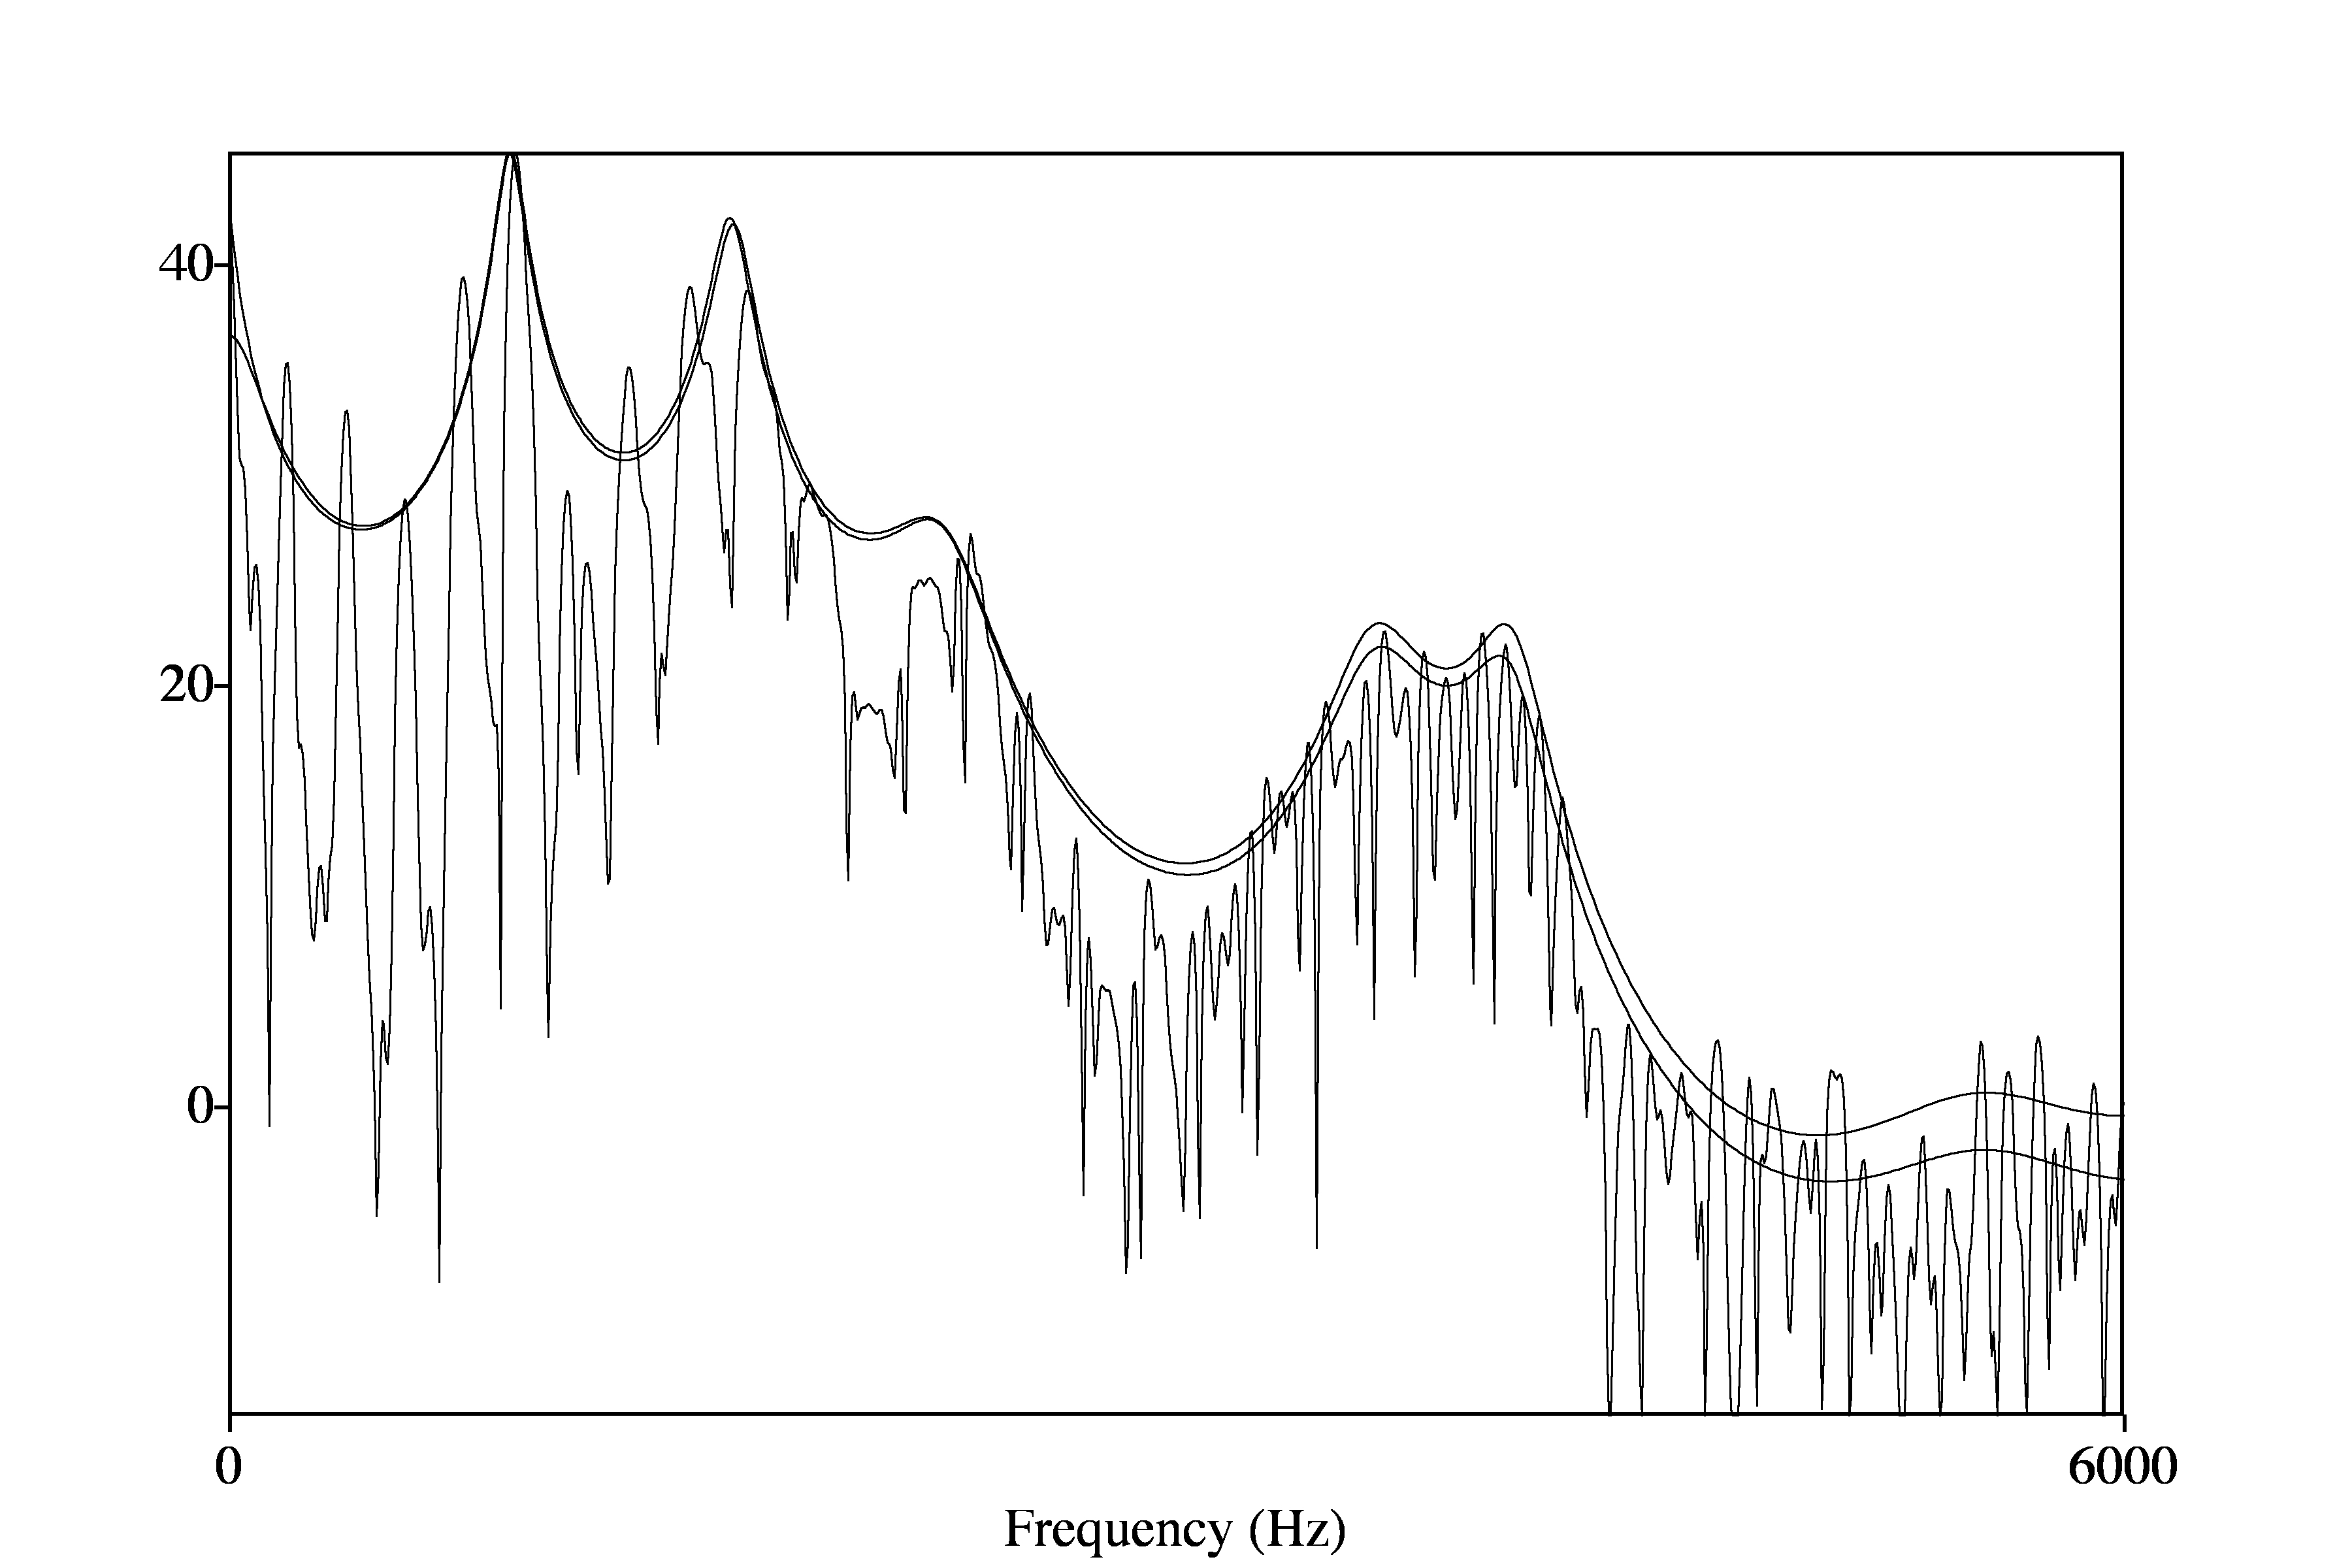
\includegraphics[width=0.75\linewidth]{figs/formants.jpg}
\caption{A Fourier spectrum overlaid with two LPC spectra. The lower one was made using the \texttt{LPC smoothing...} button, with 7 peaks requested. The upper one was made the explicit way, using 14 LPC coefficients and a window length of 0.05~s.}
\end{figure}

\noindent\textbf{Warning:} The \texttt{LPC smoothing} button is not documented in the Praat manual, so there’s no way to be sure of what it actually does. The documented way of doing this is more complicated, but for completeness:

\begin{enumerate}[label=(\alph*)]
    \item In the editor, plunk the cursor at the desired time point, make your spectral slice, and draw the resulting Fourier spectrum.
    \item Write down that time point on a piece of paper.
    \item Now, with the original Sound object selected, choose \texttt{Formants and LPC: To LPC...}. For \textit{Prediction order}, enter twice the number of peaks (formants) you want the algorithm to look for (Ladefoged, 2003, p.~123). For \textit{Analysis window duration (s)}, enter the length of the analysis window you used to do your Fourier spectrum. Click \texttt{OK}.
    \item You will see a new LPC object. With it selected, click \texttt{To Spectrum (slice)...}. For \textit{Time (seconds)}, enter the time point you wrote down, and click \texttt{OK}.
    \item You will get a new Spectrum object containing the LPC spectrum at that point. Use \texttt{Draw} to overlay it on the FFT spectrum, as before. It will be subtly different from what you got with the \texttt{LPC Smoothing...} button.
\end{enumerate}

\section{High f\textsubscript{0}s}

When f\textsubscript{0} is high, the harmonics are widely spaced and not very informative about the shape of the vocal tract’s response curve. Since the FFT algorithm is dependent on the harmonics, high f\textsubscript{0} can lead to wrong formant estimates. 

\begin{figure}[h!]
\centering
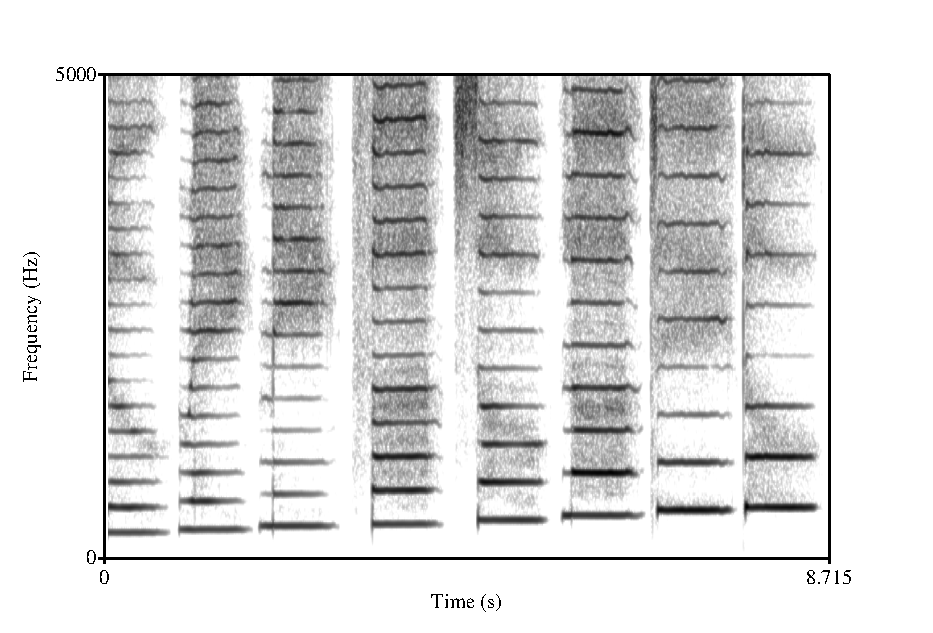
\includegraphics[width=0.75\linewidth]{figs/soprano_major.eps}
\caption{ A major scale sung by a female speaker. The first and last vowels are both [oʊ]. }
\end{figure}

The FFT spectra halfway through the two vowels show that F2 is absent in the right-hand panel, see Figure~\ref{fig:soprano_right}.

\begin{figure}[h!]
\centering
\begin{minipage}[t]{0.48\linewidth}
    \centering
    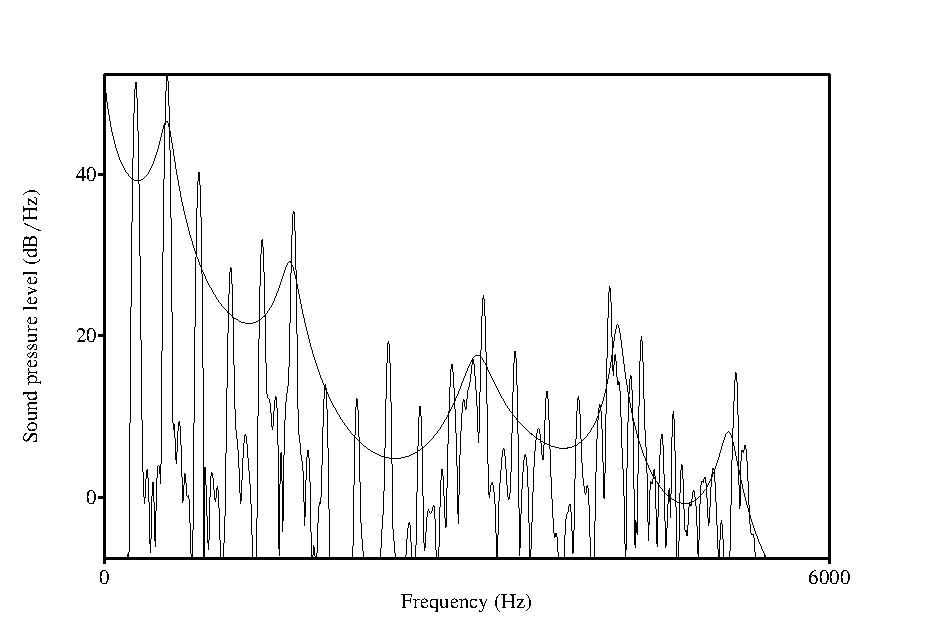
\includegraphics[width=\linewidth]{figs/sooprano_do.eps}
    \caption{FFT spectrum halfway through the first [oʊ] vowel.}
    \label{fig:soprano_left}
\end{minipage}
\hfill
\begin{minipage}[t]{0.48\linewidth}
    \centering
    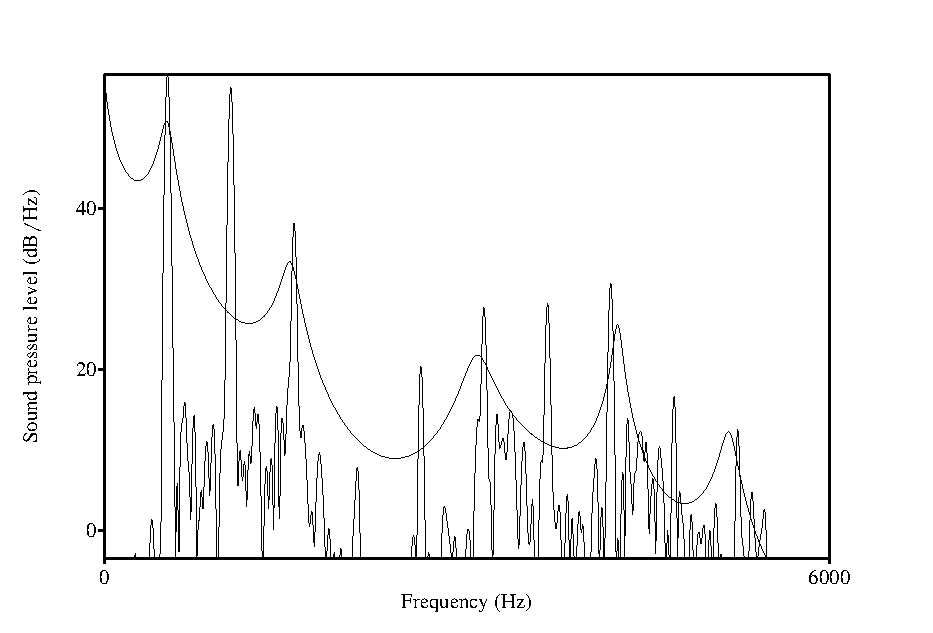
\includegraphics[width=\linewidth]{figs/soprano_do2.eps}
    \caption{FFT spectrum halfway through the last [oʊ] vowel.}
    \label{fig:soprano_right}
\end{minipage}
\end{figure}

The easiest way to avoid this problem is to avoid high f\textsubscript{0}s in the first place: Use speakers with low-pitched voices, and elicit the vowels in contexts that make a low f\textsubscript{0} likely (low tones, low pitch accents, etc.).

Sometimes it is possible to measure formants even when the harmonics are widely spaced, by looking for non-harmonic clues. Some such clues are present in this example that would allow the formants to be measured accurately even on the last vowel. What are they?

\section*{References}

\begin{itemize}[leftmargin=1.5em]
    \item Ladefoged, P. (2003). \textit{Phonetic Data Analysis}. Malden, Massachusetts: Blackwell.
    \item Thomas, E.~R. (2011). \textit{Sociophonetics: An Introduction}. Palgrave Macmillan.
\end{itemize}

%%If using linguex, need the following commands to get correct LSA style spacing
%% these have to be after  \begin{document}
    % \setlength{\Extopsep}{6pt}
    % \setlength{\Exlabelsep}{9pt}		%effect of 0.4in indent from left text edge
%%

%% Line spacing setting. Comment out the line spacing you do not need. Comment out all if you want single spacing.
%	\doublespacing
%	\onehalfspacing


%\maketitle
%\maketitleinst

% \tableofcontents

%------------------------------------
%\section{} \label{}
%------------------------------------


%------------------------------------
%\section{} \label{}
%------------------------------------


%------------------------------------
%\section{} \label{}
%------------------------------------


%------------------------------------
%\section{} \label{}
%------------------------------------


%------------------------------------
%BIBLIOGRAPHY
%------------------------------------

%\singlespacing
%\nocite{*}
% \printbibliography[heading=bibintoc]

\end{document}